\documentclass[14pt,a4paper]{extarticle}

\usepackage{fontspec}
\setmainfont{Times New Roman}
\setsansfont{Helvetica}
\usepackage{polyglossia}
\setdefaultlanguage{russian}
\setotherlanguage{english}
\newfontfamily\russianfonttt{Courier New}

\usepackage[left=30mm,right=15mm,top=20mm,bottom=20mm]{geometry}
\usepackage{setspace}
\onehalfspacing
\usepackage{indentfirst}
\setlength{\parindent}{1.25cm}

\tolerance=9000
\emergencystretch=3em
\hbadness=10000
\setlength{\overfullrule}{0pt}

\usepackage{graphicx}
\usepackage{float}

\usepackage{caption}
\captionsetup[figure]{name=Рисунок,labelsep=endash}

\usepackage{fancyhdr}
\pagestyle{fancy}
\fancyhf{}
\fancyfoot[C]{\thepage}
\renewcommand{\headrulewidth}{0pt}

\usepackage[hidelinks]{hyperref}

\usepackage{listings}
\lstset{
  basicstyle=\small\ttfamily,
  breaklines=true,
  frame=single,
  xleftmargin=1.25cm,
  numbers=left,
  numberstyle=\tiny,
  showstringspaces=false,
  tabsize=4,
}

\begin{document}

\thispagestyle{empty}
\begin{center}
\textbf{МИНИСТЕРСТВО НАУКИ И ВЫСШЕГО ОБРАЗОВАНИЯ РОССИЙСКОЙ ФЕДЕРАЦИИ}\\[0.3cm]
\textbf{УНИВЕРСИТЕТ ИТМО}\\[0.5cm]
Факультет ПИиКТ\\[1.5cm]

\textbf{\Large Лабораторная работа №2}\\[0.5cm]
\textbf{\large ASP.NET Razor Pages}\\[0.5cm]
по дисциплине <<Создание программного обеспечения>>\\[2cm]
\end{center}

\begin{flushleft}
\hspace{1.25cm}\begin{minipage}[t]{\dimexpr\textwidth-1.25cm\relax}
\textbf{Выполнил:} студент Луценко Владимир\\
\textbf{Группа:} К3420\\
\textbf{Преподаватель:} Осипов Н. А.\\
\end{minipage}
\end{flushleft}

\vfill
\begin{center}
Санкт-Петербург, 2026
\end{center}
\newpage

\tableofcontents
\newpage

\section{Введение}

Цель работы -- знакомство с технологией ASP.NET Razor Pages. В ходе лабораторной были выполнены два задания: создание простого веб-приложения с формой и разработка CRUD-приложения с базой данных.

\section{Задание 1. WebAppCoreProduct}

Создан пустой проект ASP.NET Core с поддержкой Razor Pages. В проекте реализована страница с моделью \texttt{Product}, содержащей поля \texttt{Name} и \texttt{Price}.

Добавлена форма для расчёта скидки. При отправке формы методом POST вычисляется цена со скидкой. Реализованы обработчики \texttt{OnGet} и \texttt{OnPost}, а также именованные обработчики \texttt{OnPostDiscont} и \texttt{OnPostDouble}.

Создана макетная страница \texttt{\_Layout.cshtml} с общей навигацией для всех страниц.

\begin{lstlisting}[caption={Обработчик OnPost в Product.cshtml.cs},language={[Sharp]C}]
public void OnPost()
{
    if (Price > 0)
    {
        decimal discount = Price * Discont / 100;
        Result = Price - discount;
        Message = $"Цена со скидкой: {Result:F2}";
    }
}

public void OnPostDouble()
{
    Result = Price * 2;
    Message = $"Удвоенная цена: {Result:F2}";
}
\end{lstlisting}

\begin{figure}[H]
\centering
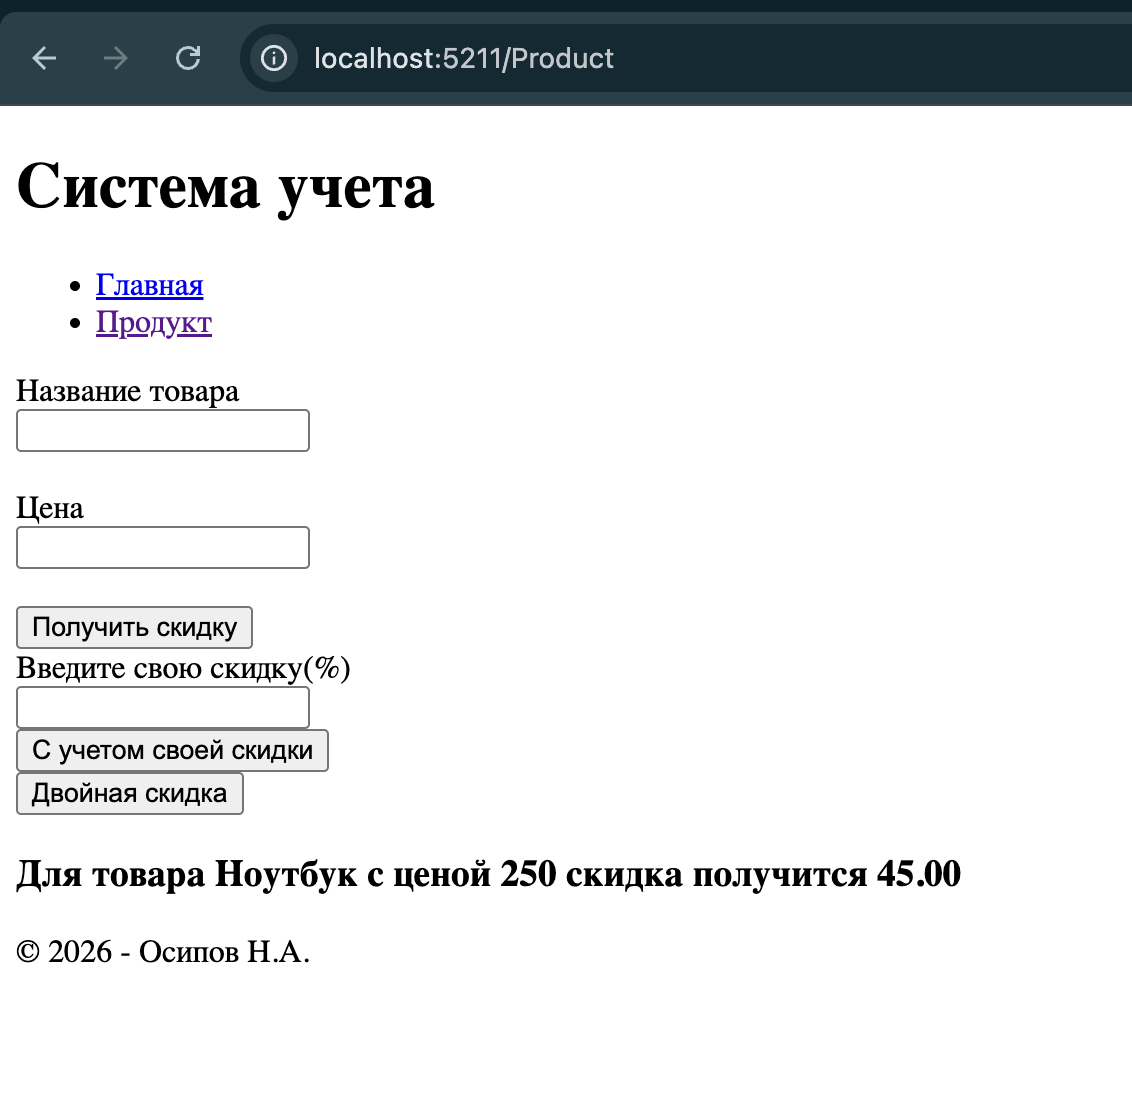
\includegraphics[width=0.6\textwidth]{../../скрины/SCR-20260328-pyro.png}
\caption{Страница Product с результатом расчёта скидки}
\end{figure}

При запуске приложения на странице \texttt{/Product} отображается форма с полями <<Название товара>> и <<Цена>>, кнопками <<Получить скидку>>, <<С учетом своей скидки>> и <<Двойная скидка>>. После отправки формы выводится результат расчёта.

\section{Задание 2. RazorPagesMovie}

Создано CRUD-приложение для управления списком фильмов с использованием Entity Framework Core и базы данных SQLite.

\subsection{Модель данных}

Модель \texttt{Movie} содержит поля с валидацией через Data Annotations:

\begin{lstlisting}[caption={Модель Movie.cs},language={[Sharp]C}]
public class Movie
{
    public int Id { get; set; }

    [StringLength(60, MinimumLength = 3)]
    [Required]
    public string Title { get; set; } = string.Empty;

    [Display(Name = "Release Date")]
    [DataType(DataType.Date)]
    public DateTime ReleaseDate { get; set; }

    [RegularExpression(@"^[A-Z]+[a-zA-Z\s]*$")]
    [Required, StringLength(30)]
    public string Genre { get; set; } = string.Empty;

    [Range(1, 100), DataType(DataType.Currency)]
    [Column(TypeName = "decimal(18, 2)")]
    public decimal Price { get; set; }

    [RegularExpression(@"^[A-Z]+[a-zA-Z0-9""'\s-]*$")]
    [StringLength(5)]
    public string Rating { get; set; } = string.Empty;
}
\end{lstlisting}

\subsection{Начальные данные и CRUD}

Для заполнения базы при первом запуске реализован класс \texttt{SeedData}. Сгенерированы CRUD-страницы: Index, Create, Edit, Details, Delete.

\subsection{Поиск и фильтрация}

На странице Index добавлен поиск фильмов по названию и фильтрация по жанру:

\begin{lstlisting}[caption={Поиск в Index.cshtml.cs},language={[Sharp]C}]
public async Task OnGetAsync()
{
    var movies = from m in _context.Movie
                 select m;

    if (!string.IsNullOrEmpty(SearchString))
    {
        movies = movies.Where(s =>
            s.Title.Contains(SearchString));
    }
    if (!string.IsNullOrEmpty(MovieGenre))
    {
        movies = movies.Where(x =>
            x.Genre == MovieGenre);
    }

    Movie = await movies.ToListAsync();
}
\end{lstlisting}

\begin{figure}[H]
\centering
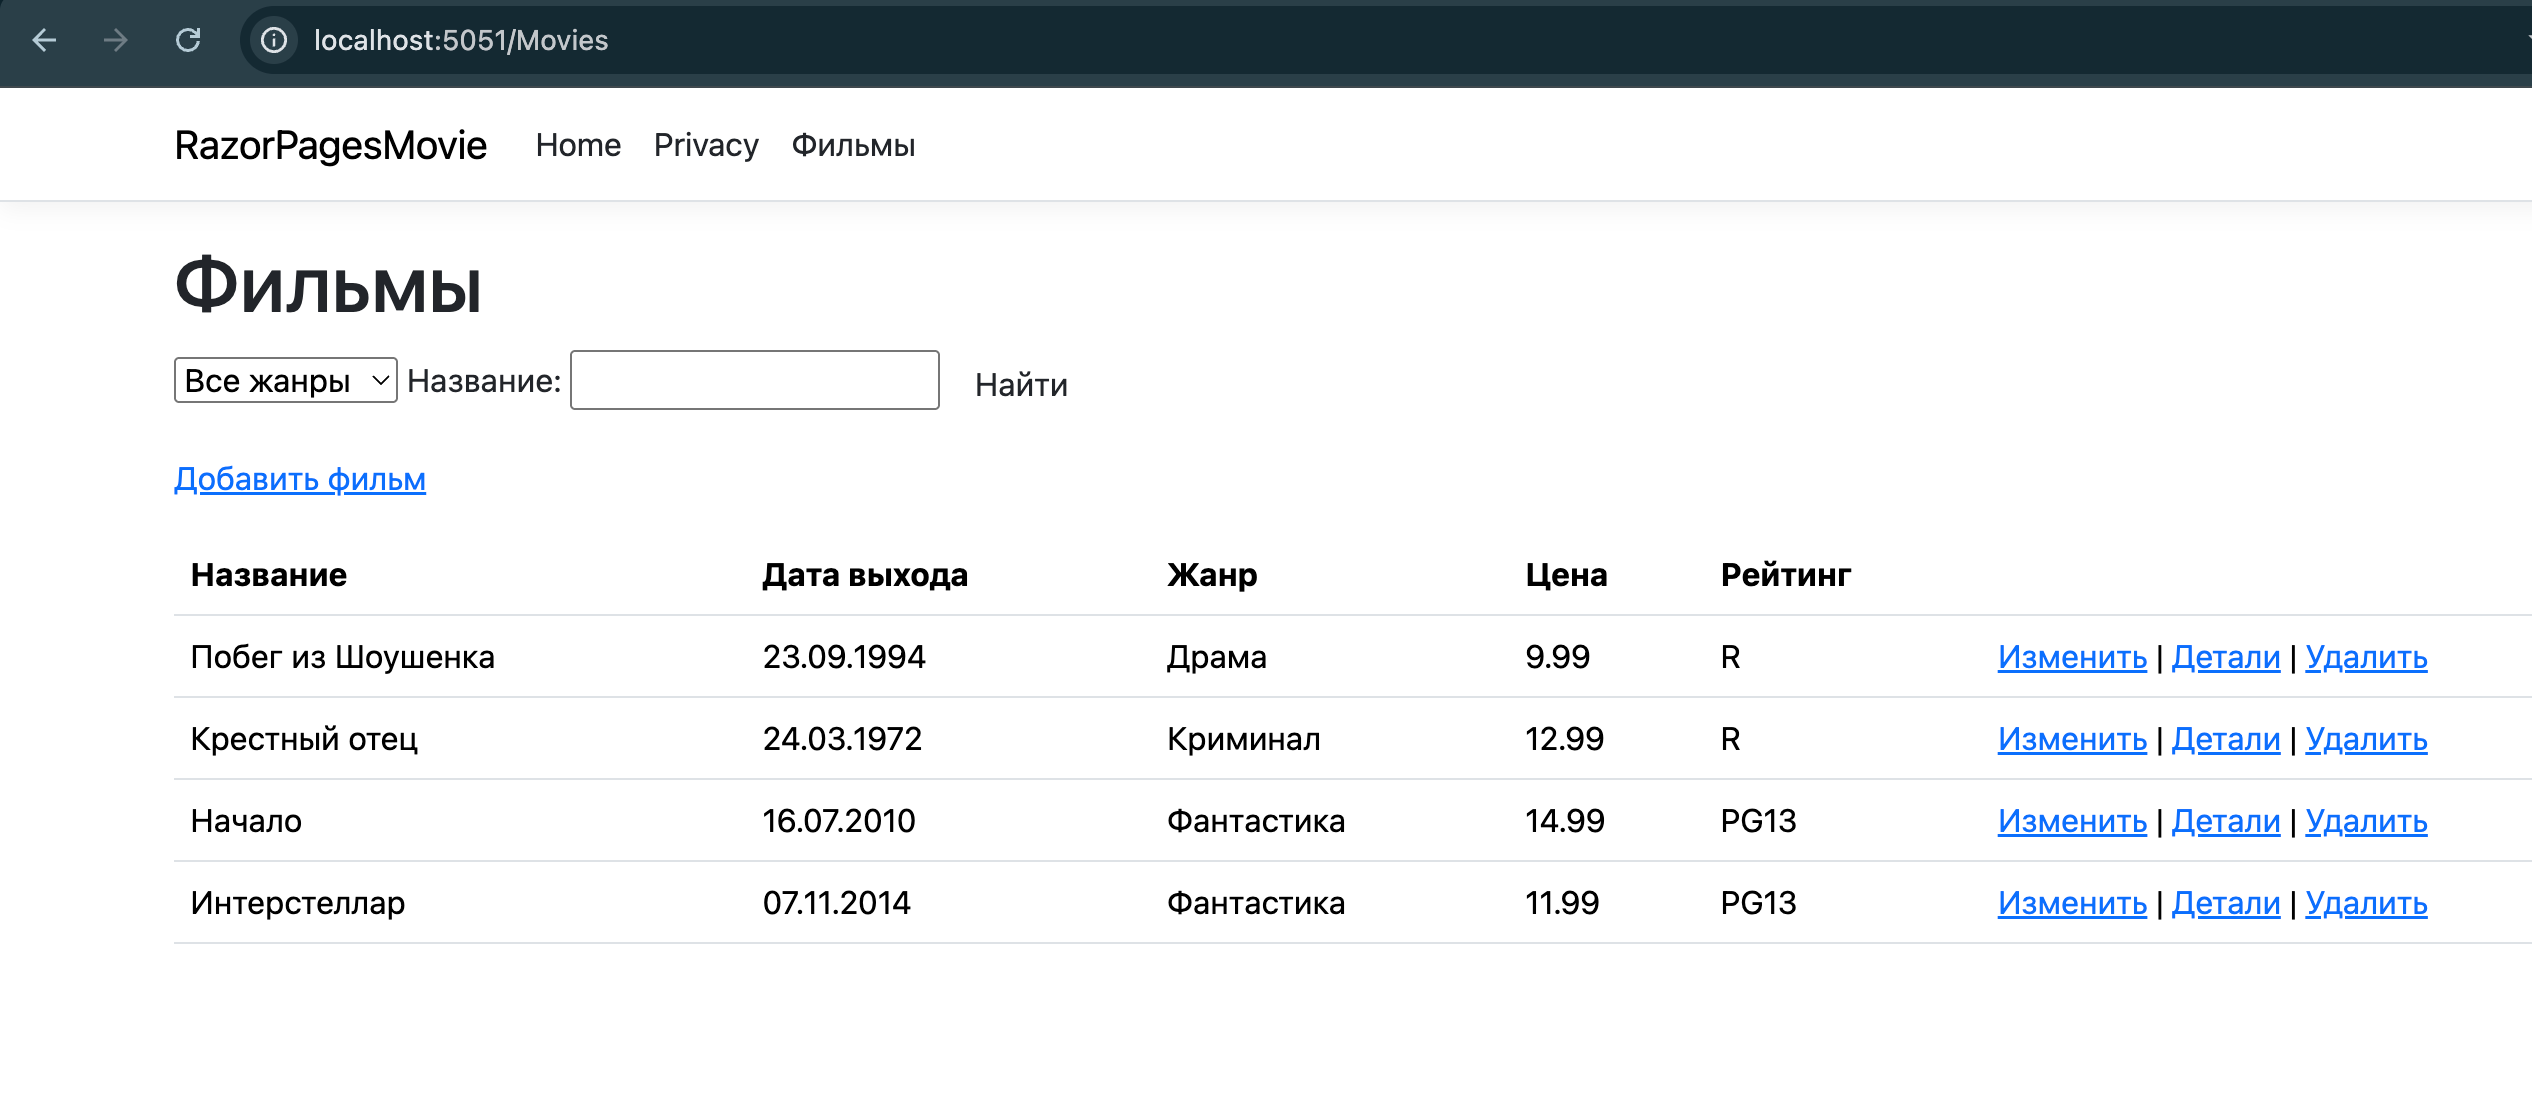
\includegraphics[width=0.8\textwidth]{../../скрины/SCR-20260328-pytt.png}
\caption{Список фильмов с поиском и CRUD}
\end{figure}

На странице \texttt{/Movies} отображается таблица фильмов с полями Название, Дата выхода, Жанр, Цена, Рейтинг. Доступен выпадающий список для фильтрации по жанру и текстовое поле для поиска по названию. Для каждого фильма доступны ссылки Изменить, Детали, Удалить.

\section{Заключение}

В ходе лабораторной работы были изучены основы ASP.NET Razor Pages: работа с формами, привязка данных, макетные страницы, Entity Framework Core, CRUD-операции, поиск и валидация. Оба приложения успешно запускаются и работают корректно.

\end{document}
